\documentclass[]{article}
\usepackage{lmodern}
\usepackage{amssymb,amsmath}
\usepackage{ifxetex,ifluatex}
\usepackage{fixltx2e} % provides \textsubscript
\ifnum 0\ifxetex 1\fi\ifluatex 1\fi=0 % if pdftex
  \usepackage[T1]{fontenc}
  \usepackage[utf8]{inputenc}
\else % if luatex or xelatex
  \ifxetex
    \usepackage{mathspec}
  \else
    \usepackage{fontspec}
  \fi
  \defaultfontfeatures{Ligatures=TeX,Scale=MatchLowercase}
\fi
% use upquote if available, for straight quotes in verbatim environments
\IfFileExists{upquote.sty}{\usepackage{upquote}}{}
% use microtype if available
\IfFileExists{microtype.sty}{%
\usepackage{microtype}
\UseMicrotypeSet[protrusion]{basicmath} % disable protrusion for tt fonts
}{}
\usepackage[margin=1in]{geometry}
\usepackage{hyperref}
\hypersetup{unicode=true,
            pdftitle={Interactive lecture module 8 and 9},
            pdfauthor={Mette Langaas},
            pdfborder={0 0 0},
            breaklinks=true}
\urlstyle{same}  % don't use monospace font for urls
\usepackage{graphicx,grffile}
\makeatletter
\def\maxwidth{\ifdim\Gin@nat@width>\linewidth\linewidth\else\Gin@nat@width\fi}
\def\maxheight{\ifdim\Gin@nat@height>\textheight\textheight\else\Gin@nat@height\fi}
\makeatother
% Scale images if necessary, so that they will not overflow the page
% margins by default, and it is still possible to overwrite the defaults
% using explicit options in \includegraphics[width, height, ...]{}
\setkeys{Gin}{width=\maxwidth,height=\maxheight,keepaspectratio}
\IfFileExists{parskip.sty}{%
\usepackage{parskip}
}{% else
\setlength{\parindent}{0pt}
\setlength{\parskip}{6pt plus 2pt minus 1pt}
}
\setlength{\emergencystretch}{3em}  % prevent overfull lines
\providecommand{\tightlist}{%
  \setlength{\itemsep}{0pt}\setlength{\parskip}{0pt}}
\setcounter{secnumdepth}{0}
% Redefines (sub)paragraphs to behave more like sections
\ifx\paragraph\undefined\else
\let\oldparagraph\paragraph
\renewcommand{\paragraph}[1]{\oldparagraph{#1}\mbox{}}
\fi
\ifx\subparagraph\undefined\else
\let\oldsubparagraph\subparagraph
\renewcommand{\subparagraph}[1]{\oldsubparagraph{#1}\mbox{}}
\fi

%%% Use protect on footnotes to avoid problems with footnotes in titles
\let\rmarkdownfootnote\footnote%
\def\footnote{\protect\rmarkdownfootnote}

%%% Change title format to be more compact
\usepackage{titling}

% Create subtitle command for use in maketitle
\newcommand{\subtitle}[1]{
  \posttitle{
    \begin{center}\large#1\end{center}
    }
}

\setlength{\droptitle}{-2em}

  \title{Interactive lecture module 8 and 9}
    \pretitle{\vspace{\droptitle}\centering\huge}
  \posttitle{\par}
  \subtitle{TMA4268 Statistical learning}
  \author{Mette Langaas}
    \preauthor{\centering\large\emph}
  \postauthor{\par}
      \predate{\centering\large\emph}
  \postdate{\par}
    \date{14 March, 2019}


\begin{document}
\maketitle

{
\setcounter{tocdepth}{2}
\tableofcontents
}
\section{8. Tree-based methods}\label{tree-based-methods}

\href{https://www.math.ntnu.no/emner/TMA4268/2019v/8Trees/8Trees.html}{Tree-based
methods} and solutions to
\href{https://www.math.ntnu.no/emner/TMA4268/2019v/8Trees/8Trees-sol.html}{RecEx}

\subsection{Topics in Module 8}\label{topics-in-module-8}

\begin{itemize}
\tightlist
\item
  Method applicable both to regression and classification (\(K\)
  classes) and will give non-linear covariate effects and include
  interactions between covariates. Based on binary splits of each
  covariate at a time.
\item
  Glossary: root, branches, internal nodes, terminal (leaf) nodes. Tree
  drawn upside down.
\item
  A tree can also be seen as a division of the covariate space into
  non-overlapping regions.
\item
  We build a tree from binary splits in one covariate at the time,
  chosen to improve some measure of error or impurity. The tree is
  created by not looking ahead - only at the current best split - thus a
  \emph{greedy strategy}.
\item
  Criterion to minimize

  \begin{itemize}
  \tightlist
  \item
    Regression: residual sums of squares
  \item
    Classification: Gini or cross entropy impurity measure or deviance
  \end{itemize}
\end{itemize}

\begin{center}\rule{0.5\linewidth}{\linethickness}\end{center}

\begin{itemize}
\tightlist
\item
  When to stop: decided stopping criterion - like minimal decrease in
  RSS or less than 10 observations in terminal node.
\item
  Prediction in terminal nodes:

  \begin{itemize}
  \tightlist
  \item
    Regression: \(\hat{y}=\frac{1}{N_j}\sum_{i: x_i \in R_j} y_i\)
  \item
    Classification: majority vote or fraction of each class in a node -
    and cut-off on probabiity.
  \end{itemize}
\item
  Grow full tree, and then prune back using pruning strategy: cost
  complexity pruning= cost function + penalty times number of terminal
  notes (hot handled in detail).
\end{itemize}

\begin{center}\rule{0.5\linewidth}{\linethickness}\end{center}

\begin{itemize}
\tightlist
\item
  From one tree to many trees= forest. Why? To improve prediction (but
  this will give worse interpretation).
\item
  Bagging (bootstrap aggregation): draw \(B\) bootstrap samples and fit
  one full tree to each, used the average over all trees for prediction.
\item
  Random forest: as bagging but only \(m\) (randomly) chosen covariates
  (out of the \(p\)) are available for selection at each possible split.
  Rule of thumb for \(m\) is \(\sqrt{p}\) for classificaton and \(p/3\)
  for regression.
\item
  OOB: out-of-bag estimation can be used for model selection - no need
  for cross-validation.
\item
  Variable importance plots: give the total amount of decrease in RSS or
  Gini index over splits of a predictor - averaged over all B trees. May
  also be calculated over randomization of OOB.
\item
  Boosting: fit one tree with \(d\) splits, make residuals and fit a new
  tree, adjust residuals partly with new tree - repeat. Three tuning
  paramteers chosen by cross-validation.
\end{itemize}

\begin{center}\rule{0.5\linewidth}{\linethickness}\end{center}

\subsection{Problems for interactive
lecture}\label{problems-for-interactive-lecture}

\subsection{Problem 1: from regions to
tree}\label{problem-1-from-regions-to-tree}

We have a classification problem with covariates (predictors)
\texttt{Sepal.Width} and \texttt{Sepal.Length} and reponse
\texttt{Species} (three species)

The graph below gives a partition of the predictor space of variables
\texttt{Sepal.Width} and \texttt{Sepal.Length}, where the observations
are shown in different colors for the different species

\subsubsection{a) From regions to tree}\label{a-from-regions-to-tree}

Sketch the classification tree corresponding to the partition. Specify
variables that are split on and an approximate value of the split point

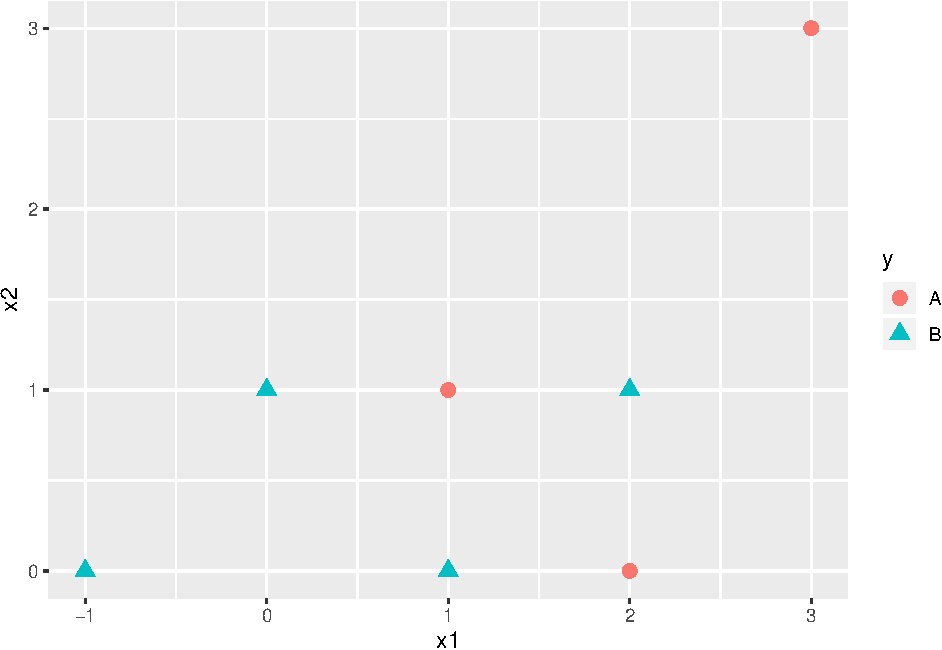
\includegraphics{89il_files/figure-latex/unnamed-chunk-1-1.pdf}

\subsubsection{b) From tree to regions}\label{b-from-tree-to-regions}

For the tree plot, draw the corresponding region plot.

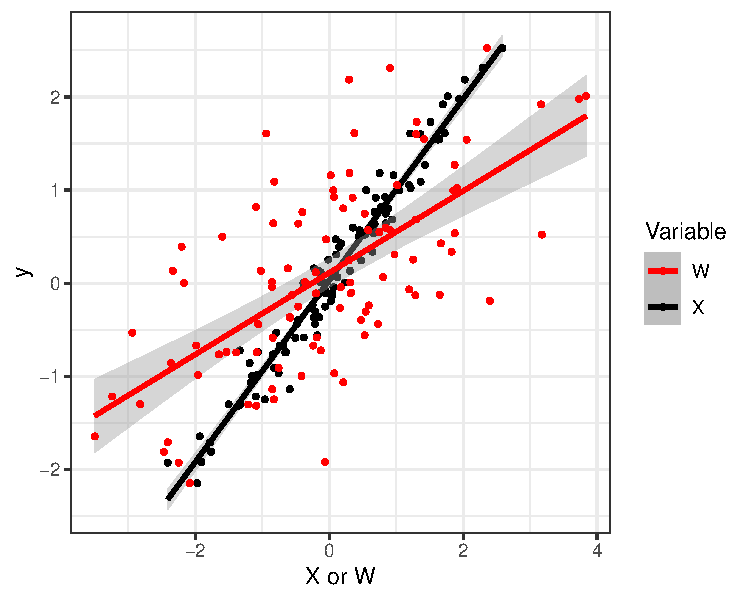
\includegraphics{89il_files/figure-latex/unnamed-chunk-2-1.pdf}

\subsection{Compulsory exercise 3 in 2018: Problem 1 on Classification
with
trees}\label{compulsory-exercise-3-in-2018-problem-1-on-classification-with-trees}

\url{https://www.math.ntnu.no/emner/TMA4268/2018v/Compulsory3.html\#problem_1_-_classification_with_trees_\%5B4_points\%5D}

\begin{center}\rule{0.5\linewidth}{\linethickness}\end{center}

\subsection{Additonal
questions/problems}\label{additonal-questionsproblems}

\begin{itemize}
\tightlist
\item
  What does it mean that a method is \emph{greedy}? Mention one greedy
  method that we have studied and explain why it is greedy.
\item
  How do we choose that we perform a split in a tree? What is the
  natural cost function for regression? For classification we focus on
  node impurity - explain one possible cost function for node impurity.
\item
  Image of tree, explain what you see. Predict the value for a new
  observation with numerical value given.
\item
  Show full tree and pruned tree and results on test set: compare and
  argument for which of the models to choose.
\end{itemize}

\begin{center}\rule{0.5\linewidth}{\linethickness}\end{center}

\begin{itemize}
\tightlist
\item
  How do we choose the number of bootstrap samples \(B\) to be used in
  bagging and random forest? What about boosting?
\item
  Why do we not have to use cross-validation to estimate error rates for
  bagging and random forest? What do we instead use, and how do we
  estimate error rates?
\item
  (MA871 exam): What is boostrapping? We have looked at boostrapping for
  finding the standard error of an estimator and for bagging and random
  forest. What is the main idea behind bagging? What is the connection
  between bagging and random forests?
\item
  For regression trees - how is a simple way to perform boosting?
\end{itemize}

\section{Learning styles}\label{learning-styles}

ACT! project - how can knowing about your learning style help your in
your study?

\url{https://innsida.ntnu.no/forms/view.php?id=221738}

\section{Compulsory exercise 2}\label{compulsory-exercise-2}

\begin{itemize}
\item
  with focus on the parts with Module 8 and 9!
\item
  \url{https://www.math.ntnu.no/emner/TMA4268/2019v/Compulsory2.html}
\item
  \url{https://www.math.ntnu.no/emner/TMA4268/2019v/CompEx2mal.Rmd}
\end{itemize}

\section{9. Support vector machines}\label{support-vector-machines}

\href{https://www.math.ntnu.no/emner/TMA4268/2019v/9SVM/9SVM.html}{Support
vector machines} and solutions to
\href{https://www.math.ntnu.no/emner/TMA4268/2019v/9SVM/9SVM-sol.html}{RecEx}.

\subsection{Topics in Module 9}\label{topics-in-module-9}

\begin{itemize}
\tightlist
\item
  SVM is a method for both classification and regression, but we have
  only studied two-class classification (classes are coded \(-1\) and
  \(1\)).
\item
  Aim: find high dimensional hyperplan that separates two classes
  \(f({\bf x})=\beta_0+{\bf x}^T \mathbf\beta=0\). If
  \(y_if({\bf x}_i)>0\) observation \({\bf x}_i\) is correctly
  classified.
\item
  Central: maximizing the distance (on both sides) from the class
  boundary to the closes observations= the margin \(M\) (maximal
  marginal classifier) - which is relaxed with slack variables (support
  vector classifiers), and to allow nonlinear functions of \({\bf x}\)
  by extending an inner product to kernels (support vector machine).
\item
  Support vectors: observations that lie on the margin or on the wrong
  side of the margin.
\end{itemize}

\begin{center}\rule{0.5\linewidth}{\linethickness}\end{center}

\begin{itemize}
\tightlist
\item
  Kernels: generalization of an inner product to allow for non-linear
  boundaries and to speed up calculations due to inner products only
  involve support vectors. Most popular kernel is radial
  \(K(x_i,x_i')=\exp(-\gamma\sum_{j=1}^p (x_{ij}-x_{i'j})^2)\).
\item
  Tuning parameters: cost and parameters in kernels - chosen by CV.
\item
  Sad: not able to present details since then a course in optimization
  is needed.
\item
  Nice connection to non-linar and ridge version of logistic regression
  - comparing hinge loss to logistic loss - but then without the
  computational advanges of the kernel method.
\end{itemize}

\begin{center}\rule{0.5\linewidth}{\linethickness}\end{center}

\subsection{Compulsory exercise 3 in 2018: Problem
3:}\label{compulsory-exercise-3-in-2018-problem-3}

\url{https://www.math.ntnu.no/emner/TMA4268/2018v/Compulsory3.html\#problem_2_-_nonlinear_class_boundaries_and_support_vector_machine_\%5B2_points\%5D}

\begin{center}\rule{0.5\linewidth}{\linethickness}\end{center}

\subsection{Additional
questions/problems}\label{additional-questionsproblems}

\begin{itemize}
\tightlist
\item
  What is a support vector?
\item
  What are differences between a maximal margin classifier and linear
  discriminant analysis classifier?
\item
  What are the main differences between the maximal margin classifier
  and the support vector classifier? Explain the concept of a slack
  variable.
\item
  What are important aspects of the support vector machine?
\end{itemize}

\section{Team kahoot!}\label{team-kahoot}


\end{document}
